\begin{figure}[H]\centering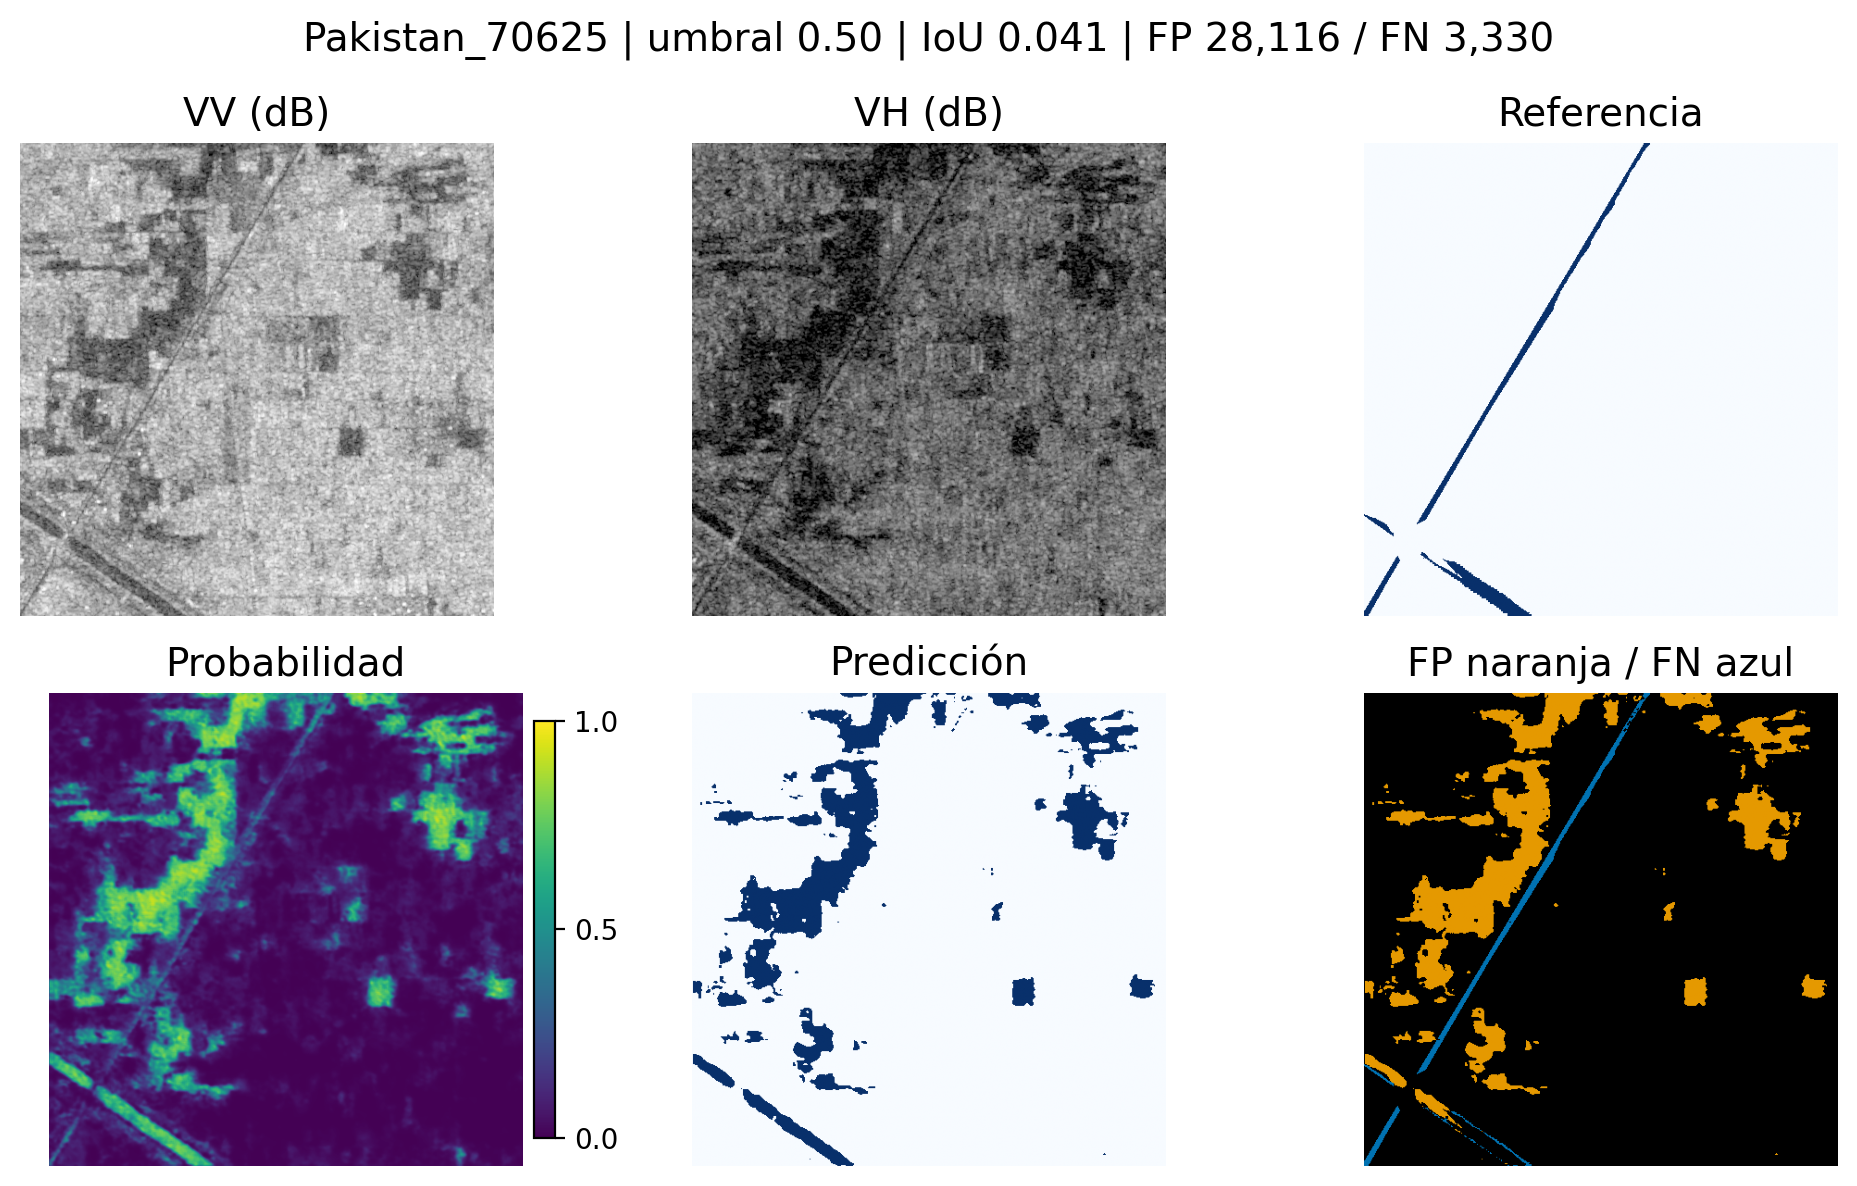
\includegraphics[width=0.96\linewidth]{figures/flood_3.png}\caption{Pakistan\_70625 (test): Se predicen manchas extensas en zonas oscuras sin agua en la referencia; el cauce diagonal fino queda parcialmente omitido.}\end{figure}
\begin{figure}[H]\centering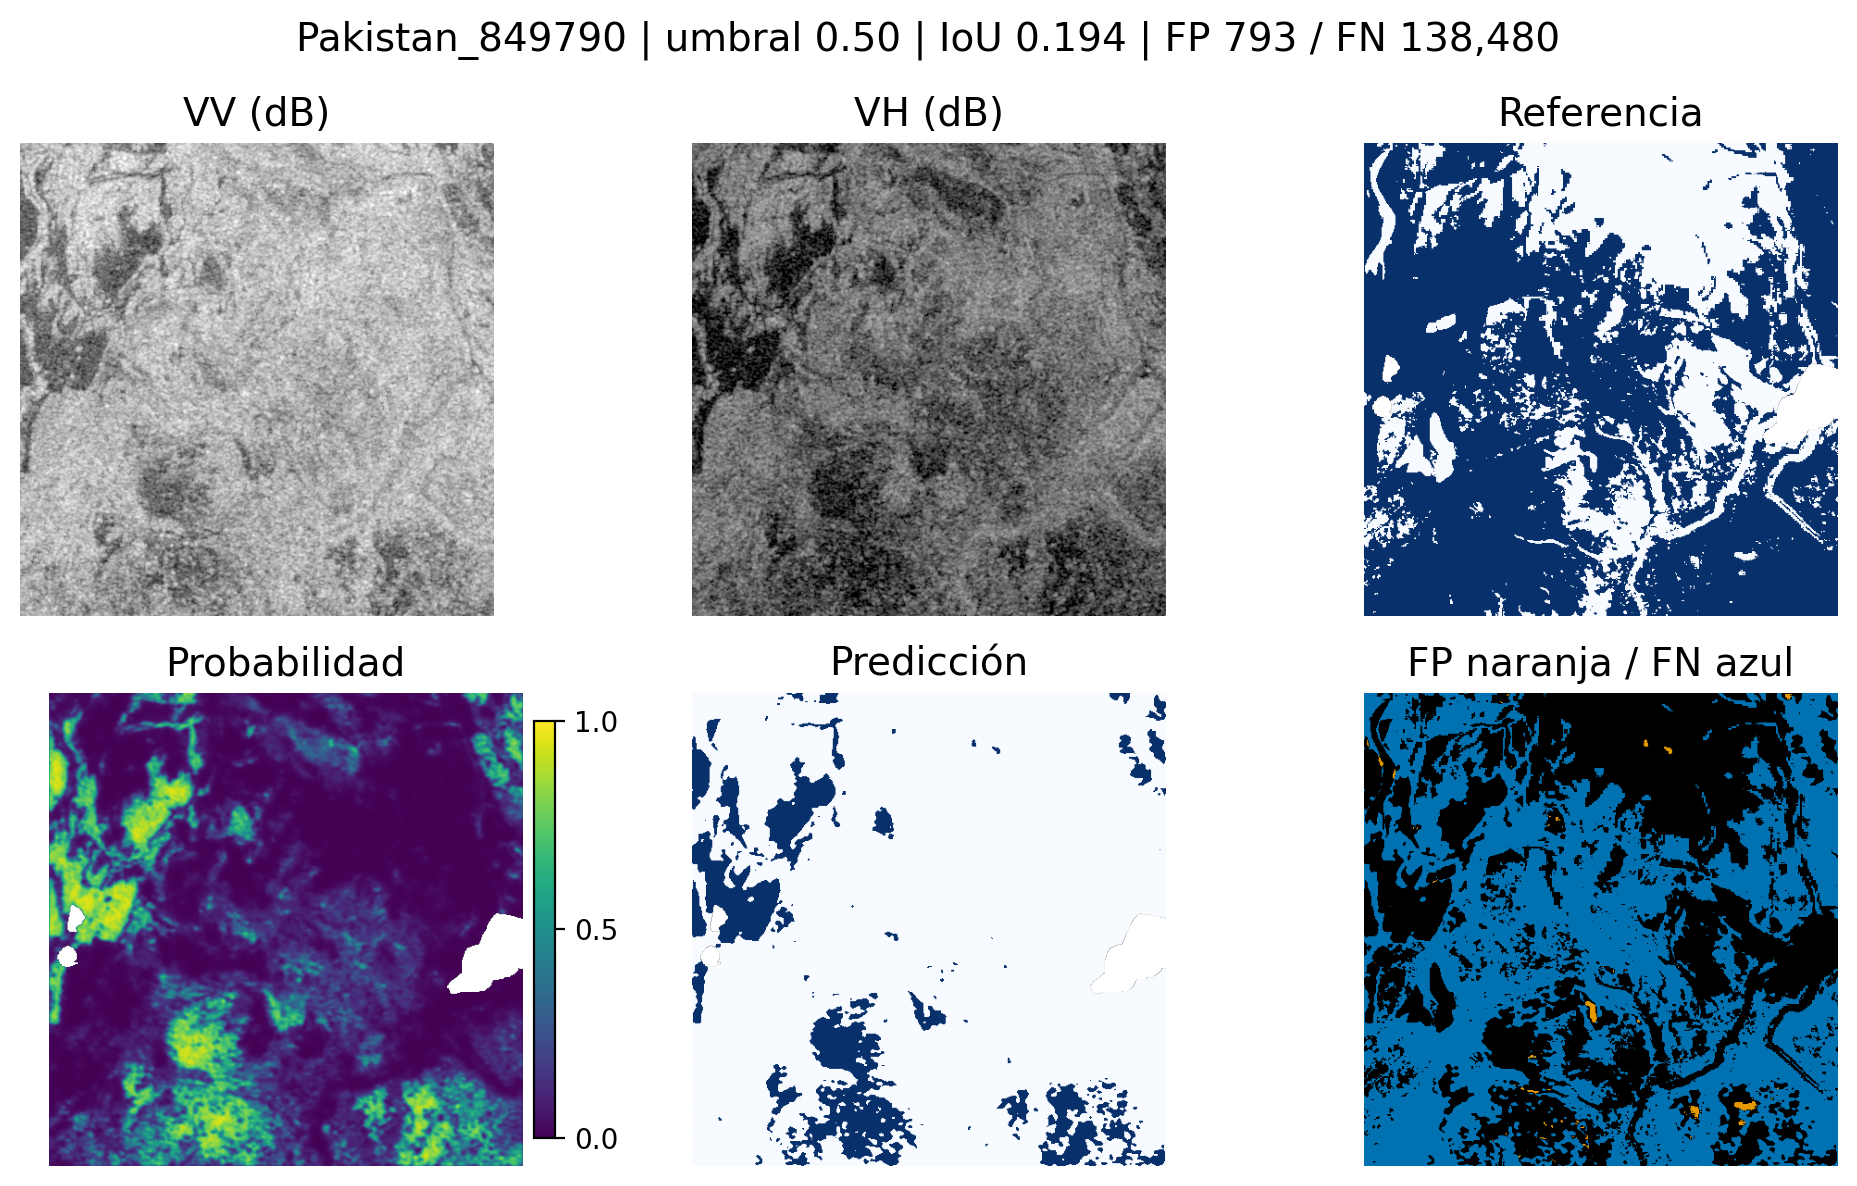
\includegraphics[width=0.96\linewidth]{figures/flood_4.png}\caption{Pakistan\_849790 (test): La referencia cubre gran parte del chip pero la predicción retiene pocas zonas oscuras; predominan falsos negativos en superficies de respuesta más alta.}\end{figure}
\begin{figure}[H]\centering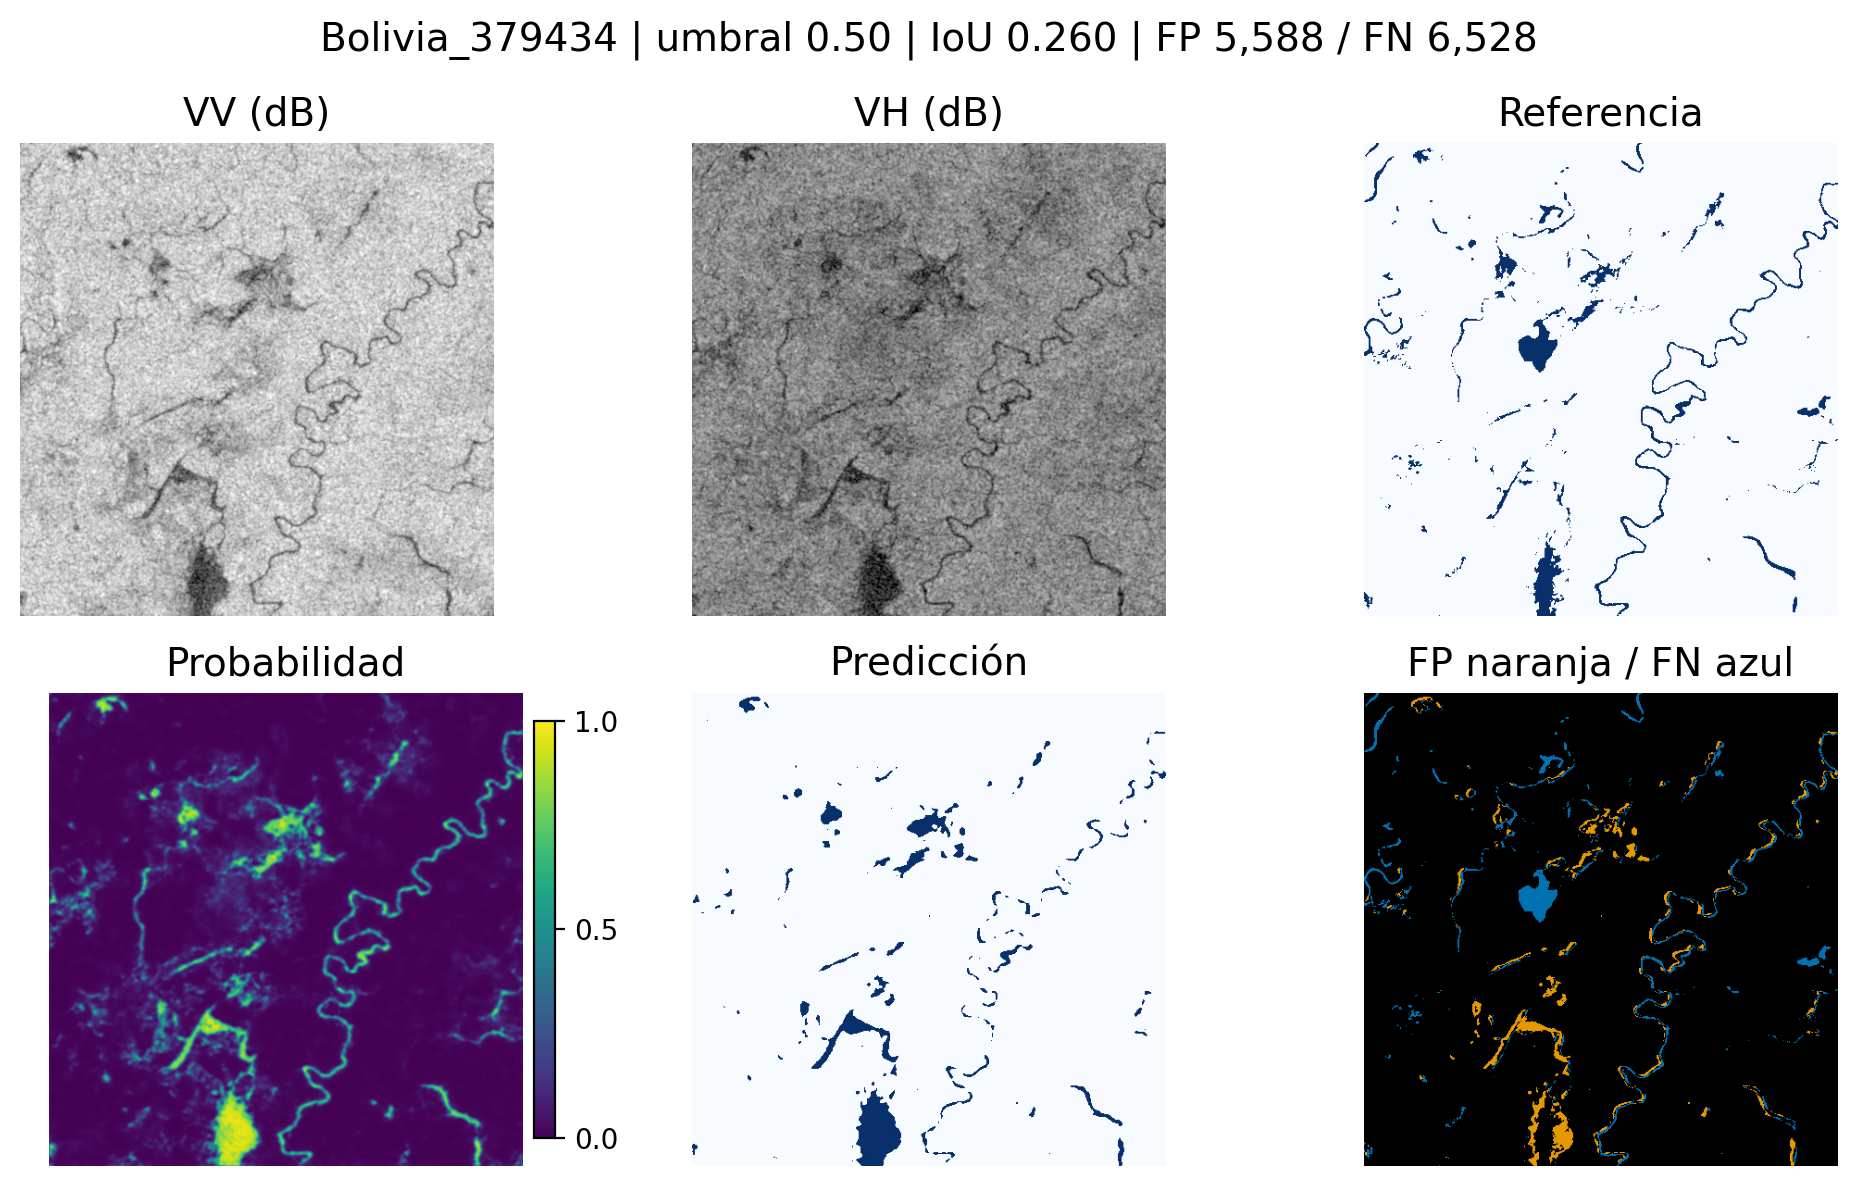
\includegraphics[width=0.96\linewidth]{figures/flood_5.png}\caption{Bolivia\_379434 (bolivia): En el cauce sinuoso derecho aparecen bandas cercanas de FP y FN y tramos fragmentados; también se omite una mancha central de agua.}\end{figure}